\chapter{Montée en compétences : programmation d'un programme simple}

\paragraph{}Afin d'apprendre à coder en C\# avec WPF, nous avons décidé de commencer par un projet bien plus modeste : le développement d'un jeu de Memory. Il s'agit d'apprendre à coder en C\# avec WPF (et donc à utiliser XAML, comme expliqué au prochain paragraphe), mais aussi de se familiariser avec l'IDE utilisé. Nous avons choisi pour cela Microsoft Visual Studio : le langage C\# a été créé pour être utilisé avec cet IDE, il permet de générer le code XAML à partir d'une interface graphique, possède des outils de déboguage très puissants et une licence est fournie aux élèves de Supélec. Comme gestionnaire de versions, nous utilisons Git.

\begin{figure}[h]
	\begin{minipage}[t]{0.5\textwidth}
		\centering
		
\includegraphics[height=1cm, width=\textwidth, keepaspectratio=true]{logoVS.png}		
	\end{minipage}
	\begin{minipage}[t]{0.5\textwidth}
		\centering
		
\includegraphics[height=1cm, width=\textwidth, keepaspectratio=true]{logoGit.png}		
	\end{minipage}
	\caption{Les logos de Visual Studio 2017 (gauche) et de Git (droite).}
	\label{fig:logos}
\end{figure}


\section{La dualité C\#/XAML}

\paragraph{}Lorsqu'un programme graphique est créé en utilisant WPF, deux langages sont utilisés. Les éléments graphiques (fenêtre, boutons, images, etc...) sont codés en XAML. Il s'agit d'un langage descriptif dérivé du XML. Il nous permet de décrire les attributs de chaque élément : par exemple, la fenêtre a un nom (utilisé pour l'appeler dans le code), un titre, une taille, une position, etc... Elle possède aussi des \enquote{children} : par exemple, un bouton. Ce bouton possède des attributs similaires, mais aussi certains attributs spécifiques, tels l'animation à effectuer lors de l'activation. Si une fonction à lancer au clic (ou lors de n'importe quel événement ayant lieu sur l'élément) peut être définie pour la fenêtre, cet attribut est obligatoire pour un bouton.

\paragraph{}Le XAML est un langage qui permet ainsi de définir rapidement une interface utilisateur, sans qu'il soit nécessaire de taper trop de code. Tous les éléments sont aussi personnalisables si nécessaire, bien que cela soit assez complexe. 

\paragraph{}Le code lui-même est écrit en C\#. Il gère toute la logique et l'interactivité du programme. Si une interactivité est nécessaire, par exemple pour changer le titre de la fenêtre au clic, il est possible de modifier tous les éléments depuis le code, d'en créer ou d'en supprimer.

\begin{figure}[H]
	\centering
	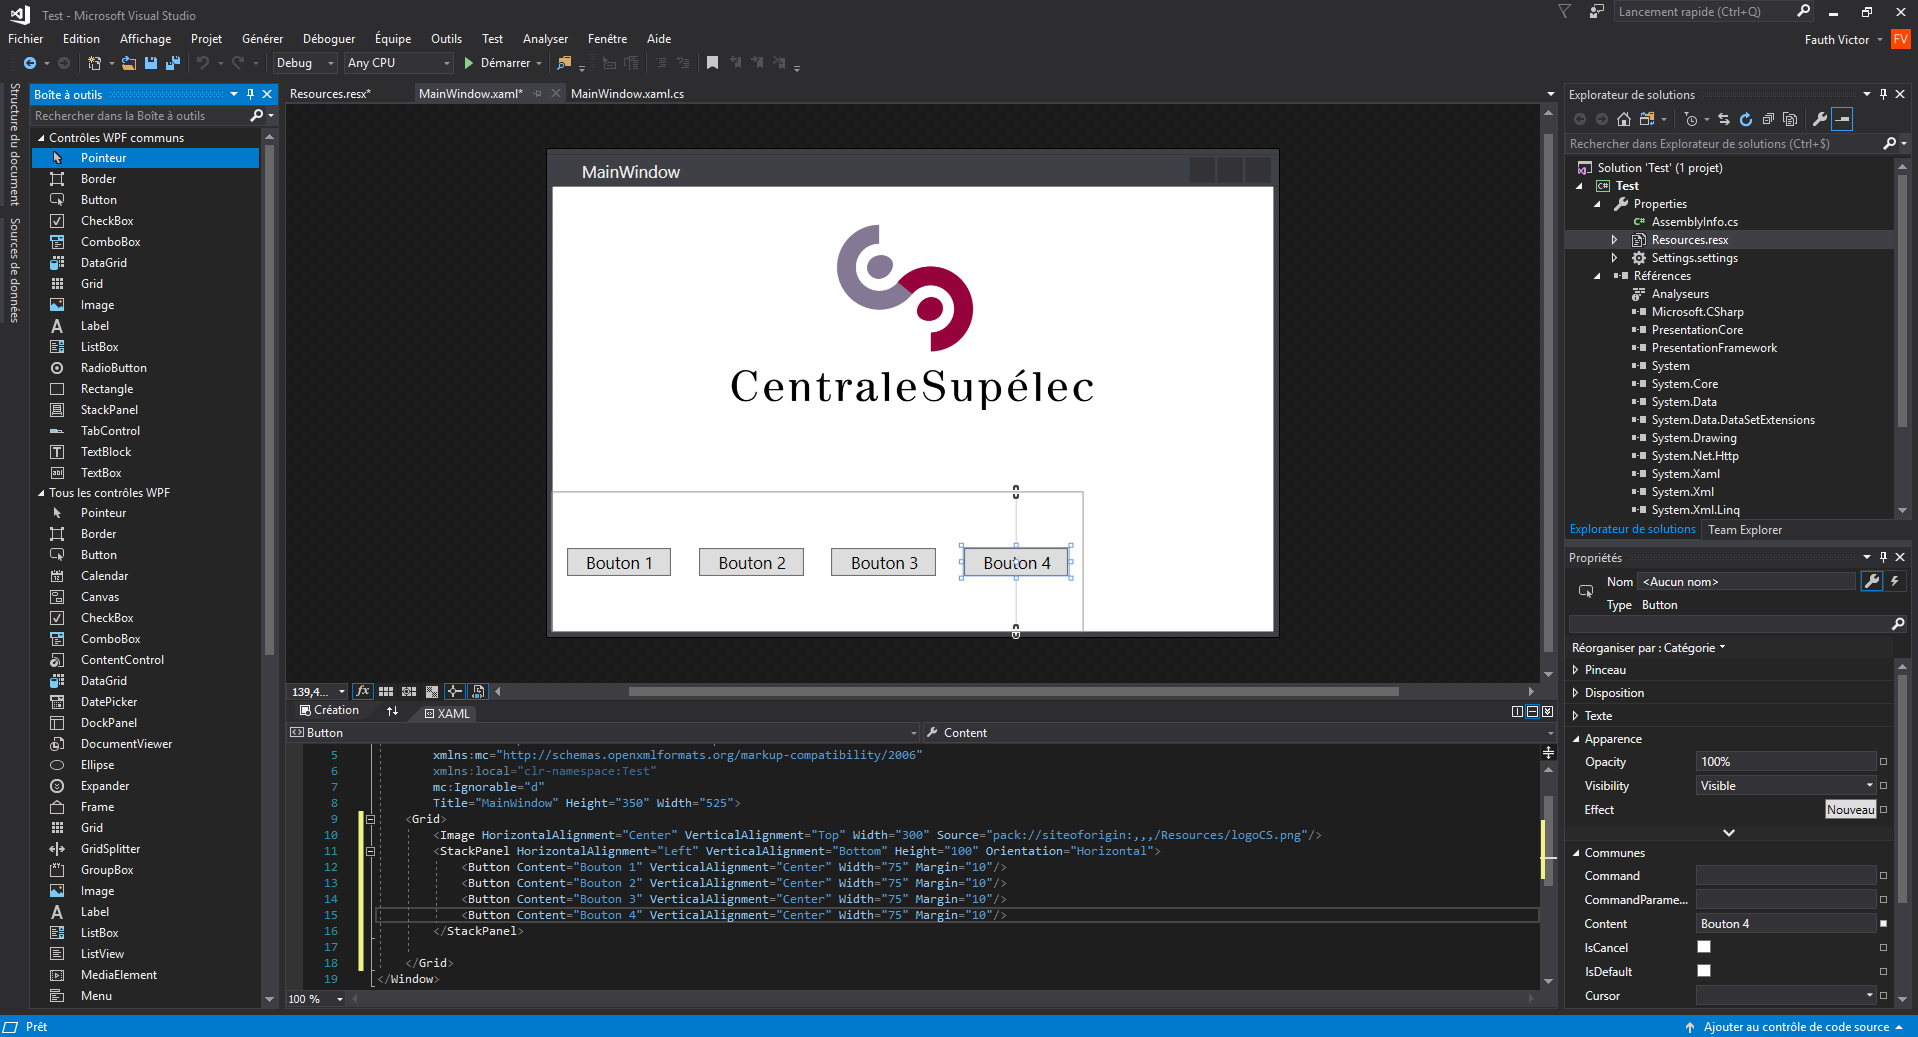
\includegraphics[width=1\textwidth]{editorXAML.png}
	\caption{L'éditeur graphique de XAML. Ici, une fenêtre avec une image et une ligne de boutons a été créée grâce à l'outil graphique, le code XAML correspondant est affiché dans la fenêtre inférieure. La fenêtre de droite permet de modifier les propriétés de l'élément sélectionné.}
	\label{fig:editorXAML}
\end{figure}


\section{Règles du jeu}

\paragraph{}Il s'agit d'un jeu très simple dans lequel un certain nombre de cartes sont posées, face cachée. Ces cartes vont par paire : chaque motif est représenté sur deux cartes. Les cartes sont posées au hasard, puis le joueur retourne deux cartes. Si elles sont identiques, la paire est retirée du jeu. Sinon, elles sont retournées face cachée, au même endroit (après un temps, ici deux secondes, permettant au joueur de mémoriser les cartes). Le jeu s'arrête lorsque toutes les paires ont été trouvées, le but étant de minimiser le nombre d'essais.


\section{Implémentation}

\subsection{Le modèle MVC}

\paragraph{}Pour coder le jeu, nous avons décidé d'utiliser l'architecture MVC (Modèle-Vue-Contrôleur). Le principe est de séparer le code en trois composantes distinctes : le modèle contient les données du programme, le contrôleur gère la logique et la vue interagit avec l'utilisateur.

\begin{figure}[h]
	\centering
	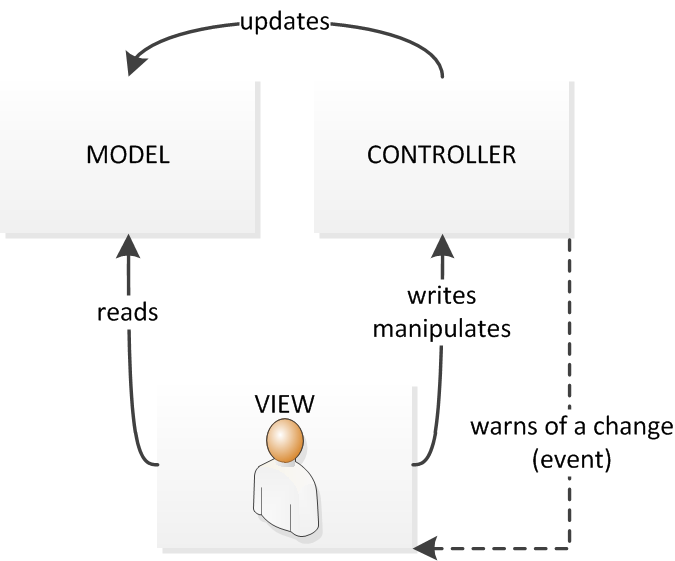
\includegraphics[width=1\textwidth]{modeleMVC.png}
	\caption{Les interactions de l'architecture MVC. Image tirée de Wikipédia.}
	\label{fig:MVC}
\end{figure}

\subsection{Le modèle}

\paragraph{}Le modèle contient l'état du jeu a un moment donné. Pour cela, nous définissons deux classes : la classe \lstinline|Card| et la classe \lstinline|Board|. 




\subsection{Le contrôleur}
\subsection{La vue}
\subsubsection{L'interface graphique statique en XAML}
\subsubsection{L'interactivité en C\#}
